\documentclass[a4paper]{article}
\usepackage[spanish,es-lcroman]{babel}
\usepackage[utf8]{inputenc}
\spanishdecimal{.}
\usepackage{bm}
\usepackage{amssymb}
\usepackage{geometry}
\usepackage{parskip}
\usepackage{graphicx}
\usepackage{listings}
\usepackage{xcolor}
\usepackage{tikz}
\usepackage{multicol}
\usepackage{enumitem}
\usepackage{subcaption}
\definecolor{mygreen}{rgb}{0,0.6,0}
\definecolor{mypurple}{rgb}{0.7,0.3,0.7}
\lstset{
	language=Python,
	backgroundcolor=\color{white},
	frame=none,
	%
	basicstyle=\tt,
	commentstyle=\itshape\color{mygreen},
	keywordstyle=\color{magenta},
	identifierstyle=\color{cyan},
	stringstyle=\color{mypurple},
	showstringspaces=false,
	%
	numbers=none,
	%	numberstyle=\color{gray},
	firstnumber = 1,
	stepnumber=2,
	tabsize =2,
	%
	columns=flexible,
	breaklines=true
}
\lstset{
     literate=%
         {á}{{\'a}}1
         {í}{{\'i}}1
         {é}{{\'e}}1
         {ý}{{\'y}}1
         {ú}{{\'u}}1
         {ó}{{\'o}}1
         {ě}{{\v{e}}}1
         {š}{{\v{s}}}1
         {č}{{\v{c}}}1
         {ř}{{\v{r}}}1
         {ž}{{\v{z}}}1
         {ď}{{\v{d}}}1
         {ť}{{\v{t}}}1
         {ň}{{\v{n}}}1
         {ů}{{\r{u}}}1
         {Á}{{\'A}}1
         {Í}{{\'I}}1
         {É}{{\'E}}1
         {Ý}{{\'Y}}1
         {Ú}{{\'U}}1
         {Ó}{{\'O}}1
         {Ě}{{\v{E}}}1
         {Š}{{\v{S}}}1
         {Č}{{\v{C}}}1
         {Ř}{{\v{R}}}1
         {Ž}{{\v{Z}}}1
         {Ď}{{\v{D}}}1
         {Ť}{{\v{T}}}1
         {Ň}{{\v{N}}}1
         {Ů}{{\r{U}}}1      
         {s̄}{{\={s}}}1
         {ñ̄}{{\~{n}}}1
         {Ñ}{{\~{Ñ}}}1
}

\newenvironment{sidefig}[1]
{\noindent\begin{minipage}[c]{#1\textwidth}}
	{\vfill\end{minipage}}
\newcommand{\herefig}[1]{%
\end{minipage}
\hfill
\noindent\begin{minipage}[c]{#1\textwidth} 
	\centering\vfill
}

\author{Celia Rubio Madrigal}
\title{Práctica 4 - GCOMP}
\date{29 de marzo de 2022}

\begin{document}
	\maketitle
	
	\tableofcontents
	
	\vfill
	
	\begin{center}
			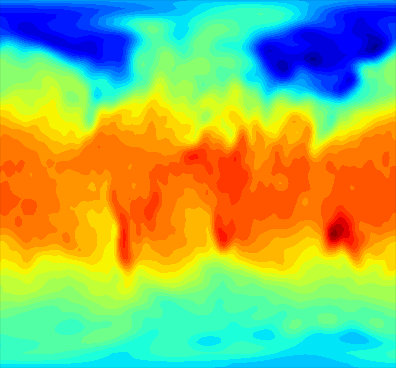
\includegraphics[width=0.5\linewidth]{portada}
	\end{center}
	
	
	\vfill
	\newpage
	
	\section{Introducción}
	En esta práctica trabajaremos con un sistema cuyos datos están tomado de la atmósfera terrestre. 
	
	Tendremos fijada una malla discreta de longitudes (variable $x$), latitudes ($y$) y niveles de presión ($p$), que no se verá modificada a lo largo del tiempo ($t$). En cada punto de la malla se habrá medido la temperatura ($T$) y la altura geopotencial ($Z$) cada día de año 2021 y parte del 2022.
	
	Se ha de observar que, por convenio, la malla no está definida a partir de alturas fijas sino de valores de presión fijos.
	
	Con estos datos, primero reduciremos el sistema en su eje temporal mediante un análisis de componentes principales, y después trataremos de predecir la temperatura de un día a partir de sus días análogos en altura geopotencial.
	
	
	\section{Material usado y metodología}
	Hemos tomado los datos del reanálisis climatológico NCEP, cuyo formato es NetCDF4. Nos proporciona una malla fija de dimensión (144,73,17) por cada día, y los valores de $T$ y $Z$ por cada uno de sus puntos.
	
	Además, hemos cambiado el sistema de referencia de las longitudes para que el 0 ($\equiv 360^\circ\equiv 2\pi$ rad) \textemdash que se corresponde geográficamente con España\textemdash~se encuentre en medio del intervalo y no al comienzo y final. Es decir, transformamos el intervalo $[0,360) \mapsto[-180,180)$ (en grados, como se encuentran los datos) o $[0,2\pi) \mapsto[-\pi,\pi)$ (en radianes).
	
	\subsection{Apartado \textit{i})}
	En el primer apartado, hemos fijado la variable $Z$ en el valor $500hPa$, y la variable $t$ en los 365 días de 2021. Así, tenemos el sistema $S_1 = \{\ a_d,\ \{Z_{x,y,p}\}_{x=1, \hspace{8pt} y=1, \hspace{4pt} p=1}^{x=144,y=73,p=17}\ \}\ \}_{d=1}^{d=365}$.
	
	A partir de él hemos estimado sus 4 componentes principales; es decir, ...%TODO. 
	Se realiza a través de la clase \verb+sklearn.decomposition.PCA+. La plantilla facilitada por el profesor proporciona dos posibles opciones para calcularlas, y debemos escoger la opción correcta.
	
	
	\subsection{Apartado \textit{ii})}
	En el segundo apartado, hemos fijado el subsistema $S_2$ donde la malla de puntos está delimitada en sus latitudes y longitudes: $x \in (−20^\circ , 20^\circ )$, $y \in (30^\circ , 50^\circ )$.
	
	Para el elemento del sistema $a_d$ con $d=``11/01/2022"$, hemos calculado los 4 elementos más análogos a él respecto a su variable $Z$. Hallamos la distancia mínima entre él y cada elemento del año 2021 usando la métrica euclídea ponderada. Los pesos distintos de 1 corresponden a la variable presión: si $p_k=500hPa$ o $p_k=1000hPa$ entonces $w_k = 0.5$, y, para el resto, $w_k=0$.
	
	Hemos creado un nuevo elemento $a_d'$ cuyos estados son la media de los estados de esos 4 elementos, tanto para su variable $Z$ como para su variable $T$, y los hemos comparado con los de $a_d$. A partir de su altura, hemos predicho la temperatura del elemento original, y así calculamos el error absoluto medio cometido de, por ejemplo, los puntos de la malla con $p=1000hPa$.
	
	\section{Resultados y conclusiones}
	\subsection{Apartado \textit{i})}
	
	La opción correcta para calcular los 4 componentes principales del sistema es la primera; es decir, la opción ``0'', que primero transpone la matriz que queremos reducir. Esto es porque el algoritmo PCA se suele aplicar para la reducción de variables de estado, pero nosotros lo usamos para la reducción del número de elementos. Podemos comprobar que la segunda opción (la ``1'', la errónea) transforma nuestra matriz de tamaño (365, 10512) en una de (365, 4).
	
	Los ratios de varianza explicada obtenidos son [0.888, 0.052, 0.005, 0.004] $\pm0.001$, cuya suma es 0.949 $\pm0.001$. Así, el porcentaje de varianza explicada es 94.5\%, una cifra considerable. Quiere decir que hemos conseguido reducir un sistema con 365 elementos en uno con 4, de forma que somos capaces de explicar el 94.5\% de la varianza de los estados originales mediante los reducidos.
	
	A continuación se muestran las gráficas de los 4 nuevos elementos obtenidos.
		
	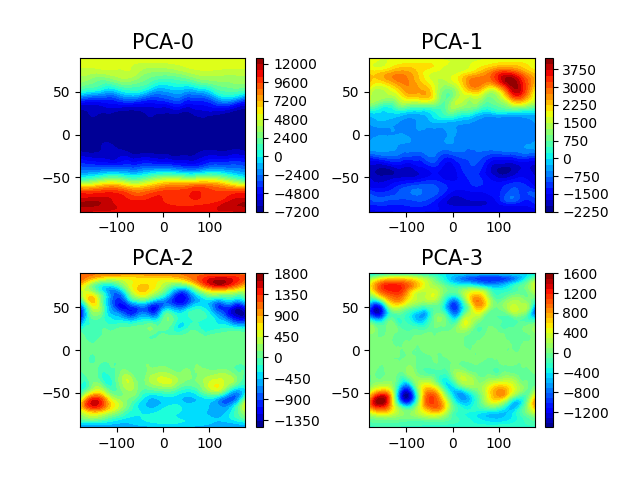
\includegraphics[width=\linewidth]{2}
	
	
	\subsection{Apartado \textit{ii})}
	Para los valores de altura geopotencial $Z$ de la malla del subsistema $S_2$ en el día $d$, y usando la distancia definida anteriormente, se han obtenido las 4 fechas más parecidas a ésta en 2021:
	23 de marzo, 16 de enero, 12 de enero y 16 de marzo.
	
	Con los valores de los estados de estos 4 elementos hemos calculado su media aritmética. A continuación se muestran, respectivamente, las gráficas de los valores reales de $Z$ ($p=500hPa$), la media de los valores más análogos, los valores reales de temperatura $T$ ($p=1000hPa$) y sus valores predichos a partir del elemento calculado.
	
	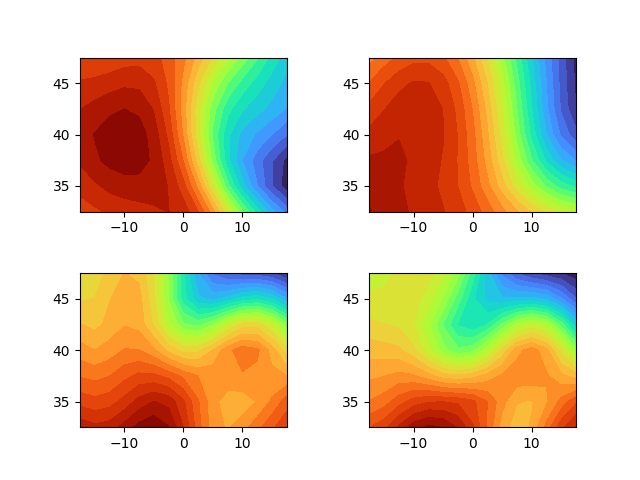
\includegraphics[width=\linewidth]{3}
	
	Se puede observar que los valores reales de temperatura y los predichos son muy cercanos, por lo que el algoritmo produce resultados satisfactorios. De hecho, para $p=1000hPa$ se obtiene un error absoluto medio de 1.419K $\pm0.001$. Este algoritmo se podría utilizar para predecir temperaturas que no supiéramos de antemano, habiéndolo ya probado en algunas que sí.
	
	En conclusión, hemos aplicado algunos algoritmos para entender los datos de un sistema altamente complejo y de persistente aplicación en el mundo real, que es la atmósfera. Hemos conseguido reducir el número de elementos del sistema, y hemos conseguido predecir los estados de un elemento a partir de otros.
	
	\newpage
	\section{Código}\label{codigo}
	
	\lstinputlisting[language=Python]{p4_rubiomadrigalcelia.py}
	
\end{document}
